\documentclass{article}
\usepackage{graphics}
\usepackage{epsfig}
\usepackage{hhline}

% define some macros:
\newcommand{\munged}{{\tt munged}}
\newcommand{\srun}{{\tt srun}}
\newcommand{\scancel}{{\tt scancel}}
\newcommand{\squeue}{{\tt squeue}}
\newcommand{\scontrol}{{\tt scontrol}}
\newcommand{\sinfo}{{\tt sinfo}}
\newcommand{\slurmctld}{{\tt slurmctld}}
\newcommand{\slurmd}{{\tt slurmd}}

\title{SLURM: Simple Linux Utility for Resource Management\thanks{
This document was prepared as an account of work sponsored by an
agency of the United States Government.  Neither the United States
Government nor the University of California nor any of their
employees, makes any warranty, express or implied, or assumes any
legal liability or responsibility for the accuracy, completeness, or
usefulness of any information, apparatus, product, or process
disclosed, or represents that its use would not infringe privately
owned rights. Reference herein to any specific commercial product,
process, or service by trade name, trademark, manufacturer, or
otherwise, does not necessarily constitute or imply its endorsement,
recommendation, or favoring by the United States Government or the
University of California.  The views and opinions of authors expressed
herein do not necessarily state or reflect those of the United States
Government or the University of California, and shall not be used for
advertising or product endorsement purposes.
This work was performed under the auspices of the U. S. Department of
Energy by the University of California, Lawrence Livermore National
Laboratory under Contract No. W-7405-Eng-48.}}

\author{Morris Jette \and Mark Grondona}

% We cheat here to easily get the desired allignment 
\date{\{jette1,mgrondona\}@llnl.gov}

\begin{document}

\maketitle

\begin{abstract}
Simple Linux Utility for Resource Management (SLURM) is an open source,
fault-tolerant, and highly scalable cluster management and job 
scheduling system for Linux clusters of thousands of nodes.  Components 
include machine status, partition management, job management, scheduling 
and stream copy modules.  This paper presents a overview of the SLURM architecture and functionality.
\end{abstract}

\section{Overview}

SLURM\footnote{A tip of the hat to Matt Groening and creators of {\em Futurama},
where Slurm is the highly addictive soda-like beverage made from worm
excrement.} (Simple Linux Utility for Resource Management) 
is a resource management 
system suitable for use on Linux clusters, large and small.  After 
surveying\cite{Jette2002} resource managers available for Linux and finding 
none that were simple, highly scalable, and portable to different cluster 
architectures and interconnects, the authors set out to design a new system.

The result is a resource management system with the following general
characteristics:

\begin{itemize}
\item {\em Simplicity}: SLURM is simple enough to allow motivated end users
to understand its source code and add functionality.  The authors will 
avoid the temptation to add features unless they are of general appeal. 

\item {\em Open Source}: SLURM is available to everyone and will remain 
free; its source code is distributed under the GNU General Public 
License\cite{GPL2002}.

\item {\em Portability}: SLURM is written in the C language, with a GNU 
{\em autoconf} configuration engine.  SLURM also supports a {\em plug-in} 
mechanism, which permits a variety of different infrastructures to be 
easily supported. The SLURM configuration file specifies which set of 
plug-in modules should be used. While initially written for Linux, other 
UNIX-like operating systems should be easy porting targets.

\item {\em Interconnect independence}: SLURM supports UDP/IP based
communication and the Quadrics Elan3 interconnect.  Adding support for 
other interconnects, including topography constraints, is straightforward 
and will utilize the plug-in mechanism described above\footnote{SLURM 
presently requires the specification of interconnect at build time}.

\item {\em Scalability}: SLURM is designed for scalability to clusters of
thousands of nodes. The SLURM controller for a cluster with 1000 nodes 
occupies on the order of 2 MB of memory and excellent performance has 
been demonstrated. Jobs may request a range of nodes, potentially 
permitting faster initiation than otherwise possible.

\item {\em Fault tolerance}: SLURM can handle a variety of failure modes
without terminating workloads, including crashes of the node running 
the SLURM controller. 
User jobs may be configured to continue execution despite the failure 
of one or more nodes. 
The user command controlling a job, {\tt srun}, may detach and reattach 
from the parallel tasks at any time. 
Nodes allocated to a job are available for reuse as soon as the allocated 
job on that node terminates. If some nodes fail to complete job termination 
in a timely fashion due to hardware of software problems, only the 
scheduling of those nodes will be effected.

\item {\em Secure}: SLURM employs crypto technology to authenticate 
users to services and services to each other with a variety of options 
available through the plug-in mechanism.  
SLURM does not assume that its networks are physically secure, 
but does assume that the entire cluster is within a single 
administrative domain with a common user base across the 
entire cluster.

\item {\em System administrator friendly}: SLURM is configured a 
simple configuration file and minimizes distributed state.  
Its configuration may be changed at any time without impacting running jobs. 
Heterogeneous nodes within a cluster may be easily managed.
Its interfaces are usable by scripts and its behavior is highly 
deterministic.

\end{itemize}

\subsection{What is SLURM?}

As a cluster resource manager, SLURM has three key functions.  First,
it allocates exclusive and/or non-exclusive access to resources 
(compute nodes) to users for 
some duration of time so they can perform work.  Second, it provides 
a framework for starting, executing, and monitoring work (normally a 
parallel job) on the set of allocated nodes.  Finally, it arbitrates 
conflicting requests for resources by managing a queue of pending work.

Users interact with SLURM through four command line utilities: 
\srun\ for submitting a job for execution and optionally controlling it
interactively, 
\scancel\ for early termination of a pending or running job, 
\squeue\ for monitoring job queues, and 
\sinfo\ for monitoring partition and overall system state.
System administrators perform privileged operations through an additional
command line utility: {\tt scontrol}.

The central controller daemon, {\tt slurmctld}, maintains the global state 
and directs operations.
Compute nodes simply run a \slurmd\ daemon (similar to a remote shell 
daemon) to export control to SLURM.  

\subsection{What SLURM is Not}

SLURM is not a comprehensive cluster administration or monitoring package.  
While SLURM knows the state of its compute nodes, it makes no attempt to put
this information to use in other ways, such as with a general purpose event
logging mechanism or a back-end database for recording historical state.
It is expected that SLURM will be deployed in a cluster with other 
tools performing these functions. 

SLURM is not a meta-batch system like Globus\cite{Globus2002}
or DPCS (Distributed Production Control System)\cite{DPCS2002}.  
SLURM supports resource management across a single cluster.

SLURM is not a sophisticated batch system.  
In fact, it was expressly designed to provide high-performance 
parallel job management while leaving scheduling decisions to an 
external entity. 

\section{Architecture}

\subsection{Node Management}

\subsection{Partition Management}

\subsection{Job Management}

\subsection{Scheduling Infrastructure}

Scheduling parallel computers is a very complex matter.  
Several good public domain schedulers exist with the most 
popular being the Maui Scheduler\cite{Jackson2001,Maui2002}. 
The scheduler used at our site, DPCS\cite{DPCS2002}, is quite 
sophisticated and has over 150,000 lines of code. 
We felt no need to address scheduling issues within SLURM, but 
have instead developed a resource manager with a rich set of 
application programming interfaces (APIs) and the flexibility 
to satisfy the needs of others working on scheduling issues.  

When jobs are submitted to SLURM they are assigned an initial 
scheduling priority through a plug-in library function. It 
maintains a priority ordered queue of pending jobs

to perform gang scheduling, namely an API 
to explicit preempt and later resume a job.

\section{Results}

\begin{figure}[htb]
\centerline{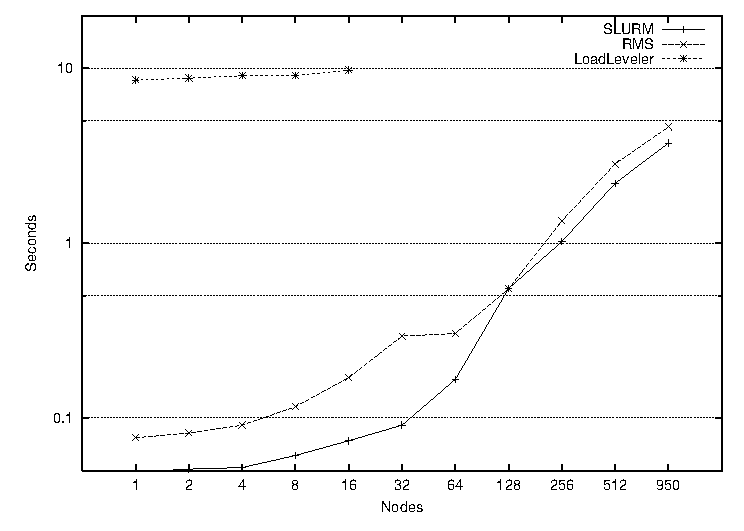
\epsfig{file=figures/times.eps}}
\caption{Time to execute /bin/hostname with various node counts}
\label{timing}
\end{figure}

We were able to perform some SLURM tests on a 1000 node cluster in 
November 2002. Some development was still underway at that time and 
tuning had not been performed. The results for executing the program 
/bin/hostname on two tasks per node and various node counts is show 
in Figure~\ref{timing}. We found SLURM performance to be comparable 
to the Quadrics Resource Management System (RMS)\cite{Quadrics2002} 
for all job sizes and about 80 times faster than IBM 
LoadLeveler\cite{LL2002} at small job sizes.
(While not shown on this chart, LoadLeveler reaches 1200 seconds to 
launch an 8000 task job on 500 nodes.)

\section{Future plans}

We expect SLURM to begin production use on LLNL Linux clusters 
starting in March 2003 and be available for distribution shortly 
thereafter. 

Looking ahead, we anticipate moving the interconnect topography 
and API functions into plug-in modules and adding support for 
additional systems. 
We plan to add support for additional operating systems 
(IA64 and x86-64) and interconnects (InfiniBand, Myrinet, and 
the IBM Blue Gene\cite{BlueGene2002} system\footnote{Blue Gene 
has a different interconnect than any supported by SLURM and 
a 3-D topography with restrictive allocation constraints.}). 
We plan to add support for suspending and resuming jobs, which 
provides the infrastructure needed to support gang scheduling. 
We also plan to support changing the node count associated 
with running jobs (as needed for MPI2).


\bibliographystyle{plain}
\bibliography{project}

\end{document}
